
\section{The Compact Muon Solenoid - CMS}

The Compact Muon Solenoid (CMS) is a multiple purpose experiment used to investigated $pp$ as well as lead-lead collisions at the LHC. It is operated by the CMS Collaborations, composed by around 200 institutes from more than 40 countries~\footnote{It is important to stress that CMS is a collaboration of institutes, not researches.}. The CMS is located in the city of Cessy, France, 100 $m$ below the surface. The CMS apparatus has an overall length of 22\unit{m}, a diameter of 15\unit{m}, and weighs 14\,000 \unit{tonnes}. A detailed description of the CMS detector, can be found in~\cite{Chatrchyan:2008zzk}. Figure~\ref{cms_sketch} presents a sketch of CMS and its subdetectors.

% cms sketch
\begin{figure}[htbp]
    \centering
    \includegraphics[width=\textwidth]{figures_and_tables/experimental_setup/cms_sketch.pdf}
    \caption{Overview of the CMS experiment and its subdetectors. Source:~\cite{Sakuma:2665537}.}
    \label{cms_sketch}
\end{figure}

The central feature of the CMS apparatus is a superconducting solenoid of 6\unit{m} internal diameter, providing a magnetic field of 3.8\unit{T}. Within the solenoid volume are a silicon pixel and strip tracker, a lead tungstate crystal electromagnetic calorimeter (ECAL), and a brass and scintillator hadron calorimeter (HCAL), each composed of a barrel and two endcap sections. Forward calorimeters extend the pseudorapidity coverage provided by the barrel and endcap detectors. Muons are detected in gas-ionization chambers embedded in the steel flux-return yoke outside the solenoid.  

The following sections describes the subdetectors, mentored above, and the CMS coordinate system, as well as some important variables.


\subsection{Coordinate system}

CMS uses a right-handed coordinate system (Figure~\ref{cms_coordinate_system}), with the origin at the nominal interaction point, the $x$ axis pointing to the centre of the LHC ring, the $y$ axis pointing up (perpendicular to the LHC plane), and the $z$ axis along the anticlockwise-beam direction. The polar angle $\theta$ is measured from the positive $z$ axis and the azimuthal angle $\phi$ is measured in the $x$-$y$ plane.

% cms coordinate system
\begin{figure}[htbp]
    \centering
    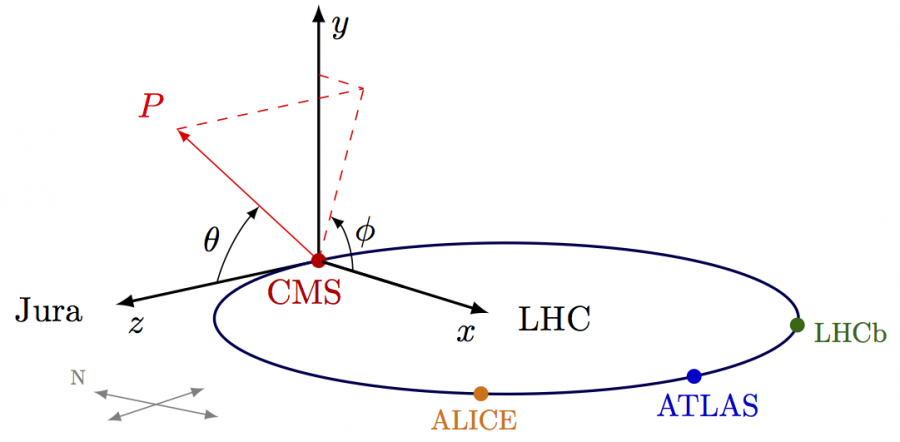
\includegraphics[width=0.7\textwidth]{figures_and_tables/experimental_setup/cms_coordinate_system.png}
    \caption{Summary of the CMS coordinate system, with respect to the LHC. Source:~\cite{cms_coordinate_system}.}
    \label{cms_coordinate_system}
\end{figure}

It is important to define some key variables for CMS, in this study. The rapidity is defined by:

\begin{equation}
    y=\frac{1}{2} \ln \left( \frac{E+p_z}{E-p_z} \right),
    \label{rapidity}
\end{equation}
where $E$ is the energy of the object and $p_z$ is the momentum of the objects along the $z$ direction. The difference between the rapidity of two objects is known for being a lorentz invariant under a boost.

A usually more suitable variable is the pseudorapidity, which is the rapidity in the relativistic limit of $E \gg m$.

\begin{equation}
    \eta = - \ln \left [ \tan \left( \frac{\theta}{2} \right)\right],
    \label{pseudorapidity}
\end{equation}
where $\theta$ is the angle between the transverse plane to the beam line ($x$-$y$ plane) and the positive $z$ direction. The convenience of using the pseudorapidity is its direct connection with the geometry of the event by the $\theta$ angle.

Spatial distance, at CMS, usually is measured based on the $\eta$-$\phi$ space. In this sense the distance $\Delta R$ between two objects is defined as:

\begin{equation}
    \begin{split}
        \Delta R &= \sqrt{(\Delta \eta)^2+(\Delta \phi)^2} \\
        & =\sqrt{(\eta_1 - \eta_2)^2+(\phi_1 - \phi_2)^2}
    \end{split}
    \label{delta_R}
\end{equation}

One last important variable is the transverse momentum component, computed as in Equation~\ref{transverse_momentum}

\begin{equation}
    \begin{split}
        p_T &= \sqrt{p_x^2 + p_y^2} \\
        & =|\mathbf{p}| \cos(\theta)
    \end{split}
    \label{transverse_momentum}
\end{equation}